%!TEX root = main_RNAPyro_JCB.tex
\section{Results}
\label{sec:results}

\subsection{Implementation}
The software was implemented in Python2.7 using the \textit{mpmath}~\cite{mpmath} library
for  arbitrary floating point precision. The source code is freely available at:

{\centering \url{https://github.com/McGill-CSB/RNApyro}\\}

The time benchmarks were performed on a MacMini 2010, 2.3GHz dual-core Intel Core i5, 8GB of RAM.
Since typical use-cases of \RNApyro require
 efficiency and scalability, we present in Table~\ref{tab:time} typical runtimes required to compute the probabilities for  every nucleotide at every positions for a vast set of parameters. For those tests,
 both the sequences and the target secondary structure were generated at random.
\TODOVlad{Add more extensive time benchmark, as a plot}


\begin{table}[t]
\begin{minipage}{.4\textwidth}
\begin{tabular}{rccc}
Length &\multicolumn{3}{c}{\#mutations}\\\cline{2-4}
		 			  & 6   &  12  & 24\\\cline{2-4}
100  				& 35s  & 238s & 1023s\\
300  			& 135s & 594s &2460s\\\cline{2-4}
		 						& 25   &    &	50		\\\cline{2-4}
500         & 5400s&       &  21003s    \\
\end{tabular}
\end{minipage}
\begin{minipage}{.59\textwidth}
\caption{Time required by the computation of probabilities. First column indicates the length and  the column indexes indicate the number
 of mutations. $\alpha$ is
set at $0.5$,  $\beta$ to $15$ and $|\Omega|=44$.}
\label{tab:time}
\end{minipage}
\SpaceCheating
\end{table}


\subsection{Error Correction in 5s rRNAs}

To illustrate the potential of our algorithm, we applied our techniques to identify and correct point-wise errors in RNA sequences
with conserved secondary structures. More precisely, we used \RNApyro to reconstruct 5s rRNA sequences with randomly distributed
mutations. This experiment has been designed to suggest further applications to error-corrections in pyrosequencing data.

We built our data set from the 5S rRNA multiple sequence alignment (MSA) available in the Rfam Database 11.0 (Rfam id: \texttt{RF00001}).
Since our software does not currently implement gaps (mainly because scoring indels is a challenging issue that cannot be fully addressed
in this work),  we clustered together the sequences with identical gap locations. From the $54$ MSAs without gap produced, we selected the
biggest MSA  which contains $130$ sequences (out of $712$ in the original Rfam MSA). Then, in order to avoid overfitting, we used \texttt{cd-hit}
\cite{Li:2006fk} to remove sequences with more than 80\% of sequence similarity. This operation resulted in a data set of $45$ sequences. 

We designed our benchmark using a leave-one-out strategy. We randomly picked a single sequence from our data set and performed $12$ random
mutations, corresponding to an error-rate of 10\%. We repeated this operation $10$ times. The value of $\beta$ was set to $15$ (larger values gave similar results). 
To estimate the impact on the distribution of the relative weights of energy and isostericity, we used 4 different values of $\alpha = {0, 0.5, 0.8, 1.0}$. 
Similarly, we also investigated the impact of an under- and over- estimate of the number of errors, by setting the presumed number of errors to 50\% (6 mutations) and 200\% (24 mutations) of their exact number (i.e. $12$).

To evaluate our method, we computed a ROC curve representing the performance of a classifier based on the mutational probabilities computed
by \RNApyro. More specifically, we fixed a threshold $\lambda \in [0,1]$, and predicted an error at position $i$ in sequence $\omega$ if and only if the
probability $P(i,x)$ of a nucleotide $x \in \{ A,C,G,U \}$ exceeds this threshold. To correct the errors we used the set of nucleotides having probability
greated than $\lambda$, that is  $C(i) = \{ x \; | \;  x \in \{ A,C,G,U \} \mbox{ and } P(i,x) > \lambda \mbox{ and }  n \neq \omega[i] \},$ where $\omega[i]$ is
the nucleotide at position $i$ in the input sequence. We note that, for lower thresholds, multiple nucleotides may be available in $C(i)$ to correct
the sequence. Here, we remind that our aim is to estimate the potential of error-correction of \RNApyro, and not to develop a full-fledged error-correction pipe-line, which  
shall be the subject of further studies. Finally, we progressively varied $\lambda$ between $0$ and $1$ to calculate the ROC curve and the area
under the curve (AUC). Our results are reported in Figure~\ref{fig:ROCall}. 

\begin{figure}
\centering
	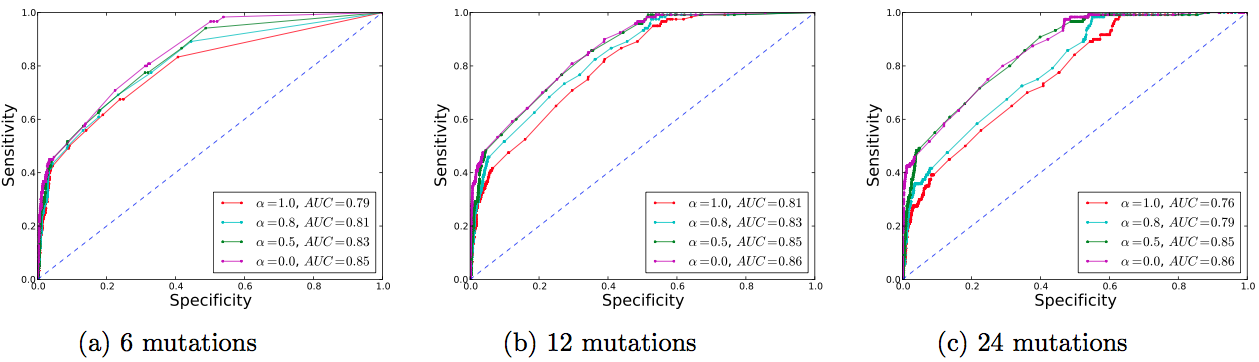
\includegraphics[width=\textwidth]{subfigs_perform.png}\\

%\begin{subfigure}[b]{0.3\textwidth}
%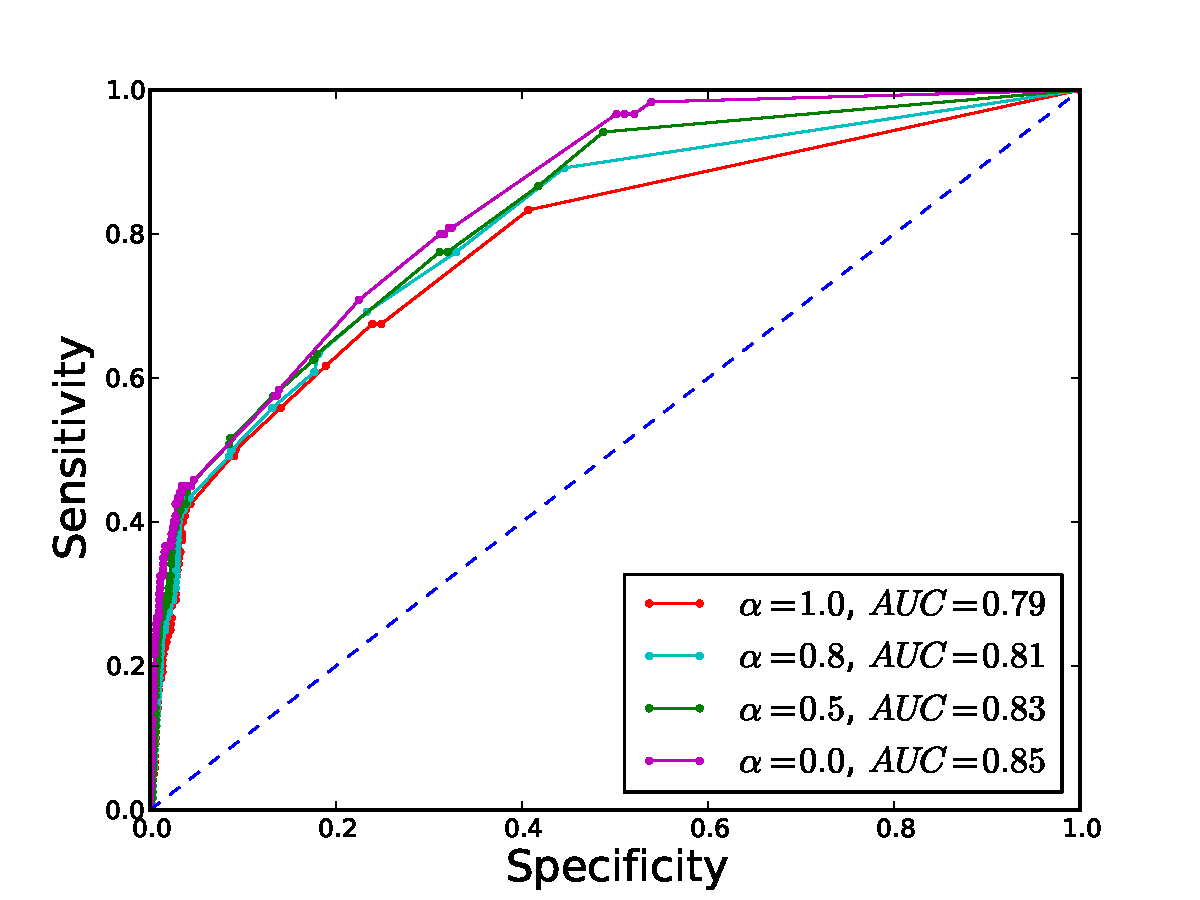
\includegraphics[width=1.2\textwidth]{figures/ROC_6.pdf}
%\caption{6 mutations}
%\label{fig:ROC6mut}
%\end{subfigure}
%\hfill
%\begin{subfigure}[b]{0.3\textwidth}
%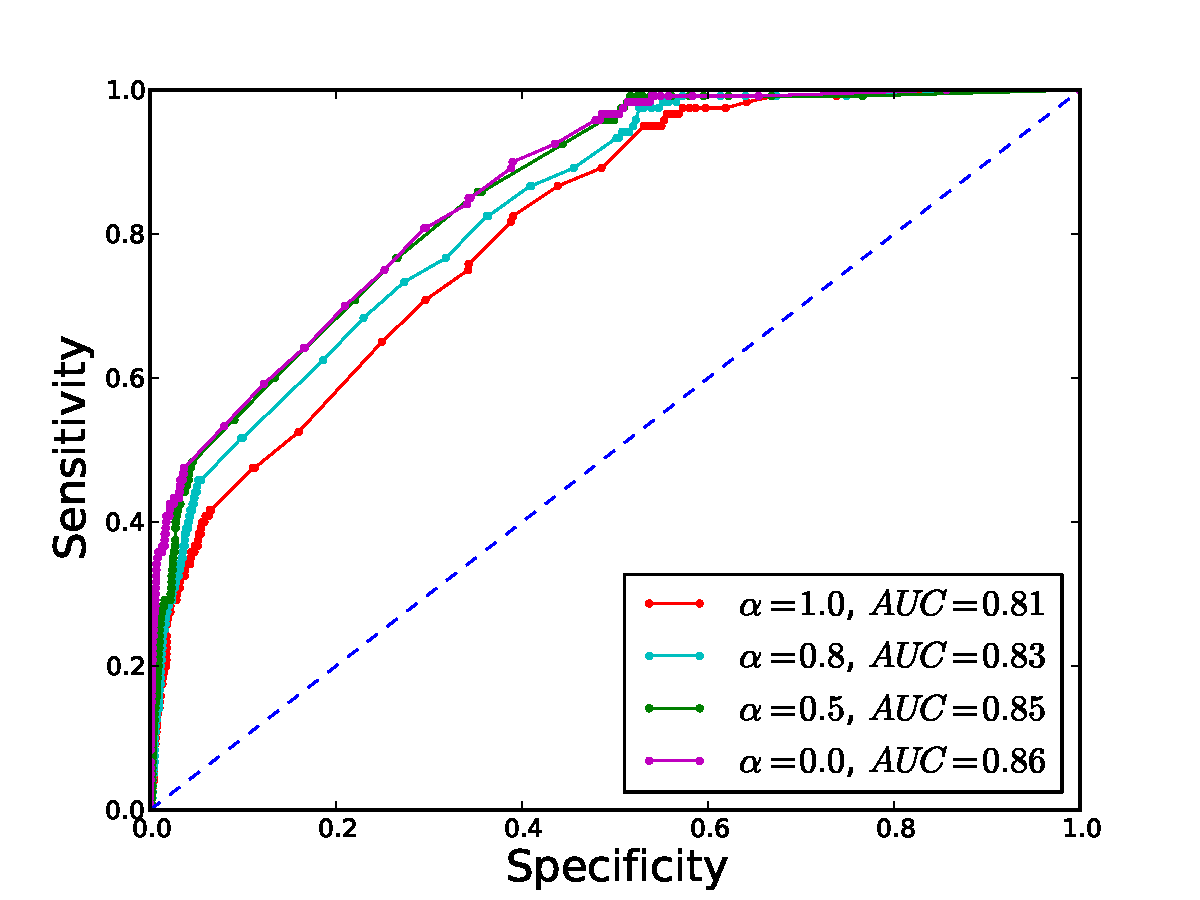
\includegraphics[width=1.2\textwidth]{figures/ROC_12.pdf}
%\caption{12 mutations}
%\label{fig:ROC12mut}
%\end{subfigure}
%\hfill
%\begin{subfigure}[b]{0.3\textwidth}
%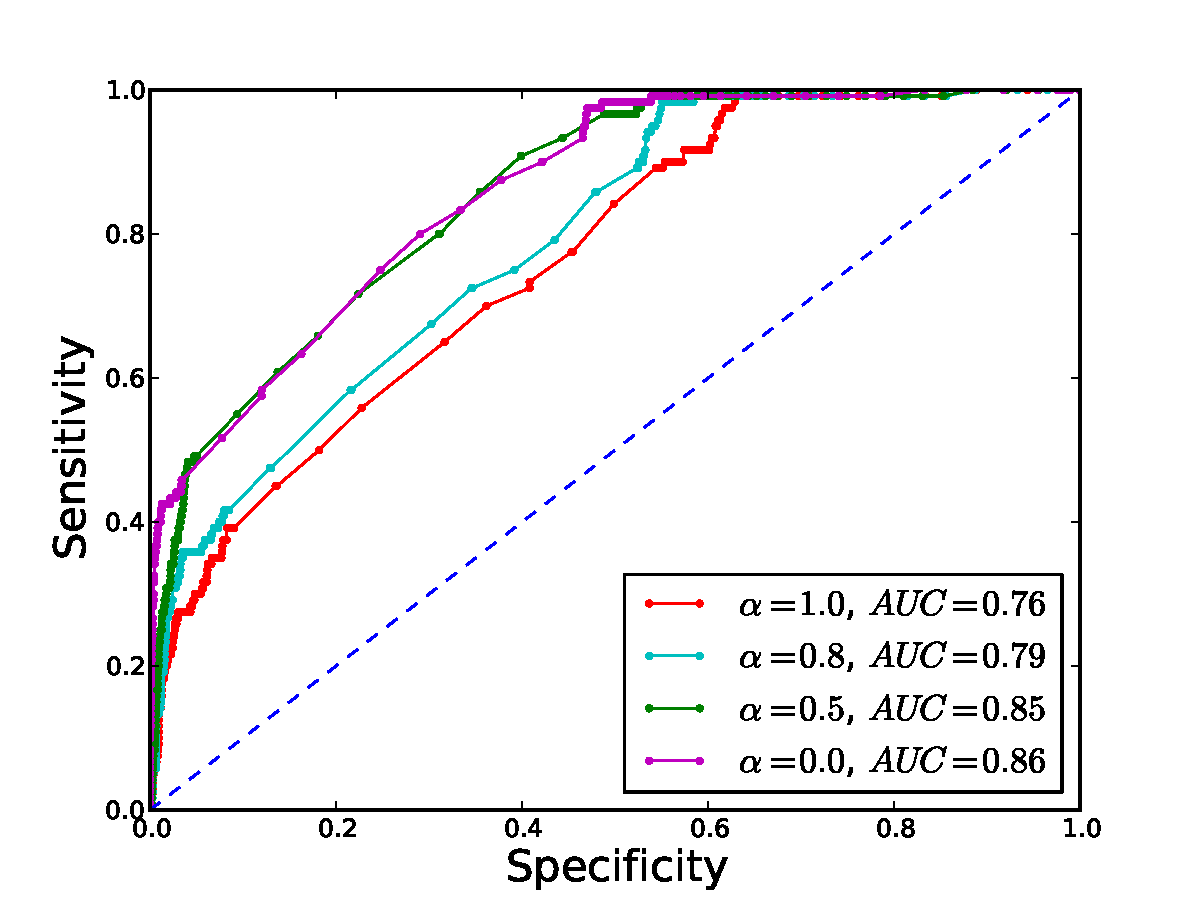
\includegraphics[width=1.2\textwidth]{figures/ROC_24.pdf}
%\caption{24 mutations}
%\label{fig:ROC24mut}
%\end{subfigure}
\caption{Performance of error-correction. Subfigures show accuracy with under-estimated error rates (6 mutations), exact estimates (12 mutations) and over estimates 
(24 mutations). We also analyze the impact of the parameter $\alpha$ distributing the weights of stacking pair energies vs isostericity scores and use values 
ranging of $\alpha=\{0,0.5,0.8,1.0\}$. The AUC is indicated in the legend of the figures. Each individual ROC curve represent the average performance over the 10 experiments.}
\label{fig:ROCall}\SpaceCheating
\end{figure}

Our data demonstrates that our algorithm exhibits interesting potential for error-correction applications. First, the AUC values (up to $0.86$) indicate that a
signal has been successfully extracted. This result has been achieved with errors in loop regions (i.e. without base pairing information) and thus suggests
that correction rates in structured regions (i.e. base paired regions) could be even higher. Next, the optimal values of $\alpha$ tend to be close to $0.0$. This 
finding suggests that, at this point, the information issued from the consideration of stacking energies is currently modest. However, specific examples showed improved performance
using this energy term. Further studies must be conducted to understand how to make the best use of it. Finally, our algorithm seems robust to the number of
presumed mutations. Indeed, good AUC values are achieved even with conservative estimates for the number of errors (c.f.~50\% of the errors, leading to 
Fig.~\ref{fig:ROCall}(a)), as well as with large  values (cf~200\% of the errors  in Fig.~\ref{fig:ROCall}(c)). It is worth noting that scoring schemes giving a larger weight on
the isostericity scores (i.e. for low $\alpha$ values) seem more robust to under- and over-estimating the number of errors.




